\documentclass[a4paper,12pt]{article}

% Språkinställning
\usepackage[utf8]{inputenc}
%\usepackage[swedish]{babel}

% Bild packages 
\usepackage{graphicx}
\usepackage{epstopdf}
% wrapping
\usepackage{wrapfig}
% Bild inställningar
\epstopdfsetup{outdir=./}
\graphicspath{img/}


\usepackage[linktoc=all]{hyperref}
\hypersetup{
    colorlinks,
    citecolor=black,
    filecolor=black,
    linkcolor=black,
    urlcolor=black
}


% ToDo
% [] Remove all forms of "me"
%   [] Introduction
%   [x] Theory
%   [] Method
%   [] Result
%   [] Analysis and discussion







\begin{document}


\title{Projectreport\\ 
       \small{Computergame}}
\author{Johan Bjäreholt\\
       \small{Polhemskolan TE3E}}
\date{2014-01-28}

\maketitle

\newpage

\section{Abstract}

%• Abstract 
%Abstract är en sammanfattning på engelska. En sammanfattning eller ett abstract är fristående från rapporten. Läsaren ska utifrån din sammanfattning kunna förstå innehållet utan att ha läst hela rapporten. Utformningen ska vara entydig och täcka innehållet utan att var för detaljerad.
%Avsikten med sammanfattningen är att ge läsaren en bild av hela rapportensamt möjlighet att avgöra om hen har intresse av att läsa vidare. Sammanfattningen ska innehålla en mycket kortfattad presentation av följande:
%Slutsatserna
%Vad arbetet handlarom
%Metoder som använts vid undersökningen 
%De viktigaste resultaten 
%Syftet med undersökningen
%Sammanfattningen bör omfatta max en halv sida, skriven i löpande text. 
%Även om sammanfattningen placeras först i rapporten är det lämpligt att skriva den sist, när du är färdig med resten av rapporten.
%Anledningen till att sammanfattningen skrivs på engelska är förberedelse för Högskolan.



\clearpage

%• Innehållsförteckning
%I innehållsförteckningen ska rapportens alla rubriker vara förtecknade med sidhänvisning. Innehållsförteckning genereras automatiskt i Word, om alla rubriker markeras som ”Rubrik” och alla sidor är numrerade.

\setcounter{tocdepth}{3}
\tableofcontents
 
\clearpage

\section{Introduction}
%• Inledning 
%Inledning ska innehålla en kort bakgrund samt syfte och frågeställningar, och avgränsningar.
%I inledningen presenterar ni frågeställningen eller problemställningen för läsaren. Inledningen ska även ge en bakgrund till problemet, er hypotes på förväntat resultat/samband.
%Syftet ska vara tydligt preciserat med vad som ska undersökas eller uppnås. Forumlera några frågeställningar som är kopplade till syftet.
%Avgränsningar är viktigt för att precisera syftet och tydliggöra vad din rapport har för avsikt att handla om. På det sättet förekommer man också kritik. Avgränsningar är ett förtydligande på vad arbetet bakom rapporten fokuserat på och vad ditt arbete inte omfattar.
%Det är viktigt att ha en bra, välskriven och intresseväckande inledning. Det är här du introducerar läsaren till ditt tänk och lyfter dina frågeställningar. Den ska vara välformulerad och uppta ungefär en sida av rapporten. 


% Project question and clear aim
%   Clear and multiple questions are good to have, and they have to be clear
% This gymnasium projects goal is to learn and make a robust base for a 2d platform game.
What does the design of a game look like abstractly in code and how does everything work together?
What are some nice architectual code designs and how do i implement them properly?
These are questions i think are very interesting and only have scraped the surface of before, and therefore have decided to learn how this works in depth with this project.

% What i am going to learn
The aim of the making of this game is not to make a good looking and fun computer game, but to learn how to make a extensive and well made code base with a test game made on top of it.
This is because i am not interested in learning the aesthetics of game making, but how to write the base code for a game.
% Description of my boundries
This means that i will avoid doing as much graphical and musicial work as possible and focus on the technology underneath this such as physics, world creation, character saving etc.
This will make the project more scientific and more interesting to analyze around when the project is done.

% Project aim and questioning of what will be hard and easy
A schedule has been made to 


\subsection{Recommended reading}
% What you need to know to fully understand the report
There is terminology and a few concepts that will repeatedly be mentioned in this report.
Most of the report will still be understood by the average person even if they are not experienced in programming and game making, but to fully understand some parts of the report (especially the analisys), you will have to either 


\clearpage

\section{Theory}
%• Teori (Teoretisk bakgrund)
%Under rubriken ”Teori” tar du upp saker som är relevanta för rapporten. Teorin är det som lägger grunden för diskussionen, så att allt du tar upp i teorin måste du återknyta till i diskussionen. På samma vis får du inte ta upp något i diskussionen som du inte tidigare har lagt grunden för och har stöd för i teoridelen.
%Om det finns olika sätt att tolka begrepp är det viktigt att du klargör hur du i din rapport använder begreppen.
%I detta avsnitt refererar du tidigare undersökningar, teorier, fakta, forskningsresultat och andra vetenskapliga artiklar/rapporter. Glöm inte att göra löpande källhänvisningar, se bilaga 1. 
%Tänk på att vara källkritisk.


% Technologies
When considering on how to actually make the game, i decided to use technologies i already knew how to use and was familiar with. 
This resulted in a combination of the programming language Python and the game library PyGame, which are are both designed very concise so i've been able to write more effective code on less amount of lines and therefore saving time which is crucial on a one man project.

% Focus
The focus of this project is to learn how to create a advanced, flexible and stable game framework.
The aim is not to add lots of game elements and make it fun, but is simply a proof of concept on how to make a good game engine.
Consicely, it's about features and not content.

% Difficulties
There are a few issues that are known that might be encountered. First off, writing a game is difficult and takes more time than people usually thinks. To explain everything the game does in code is alot of work, even though some of it might be very simple.
Secondly, i chose a high level language which is efficient to write, but as all high level languages it is slow to execute.  



\subsection{Planning, Ambition and Time Estimation}

By estimating how efficient my coding was the first weeks of my project, i could estimate and plan what i would be able to implement until the completion date.
Since the focus was on the engine, there were a few specific things included in my engine that are usualy not present in simple games as this.

The first is my menu system.
I want to be able to easily and efficiently create a menu, and make the code easy to understand to others if they would like to base their own game on my code.

The others are more game centric to make it feel premium.
Physics are important to make the game dynamic, and some extra things that would improve but not as important are multiplayer, character customization and easy world creation.

These are my ambitions,


\subsection{Software}

\subsubsection{Python}
\begin{wrapfigure}{r}{0.4\textwidth}
    \vspace{-30pt}
    \begin{center}
    
\includegraphics[width=0.38\textwidth]{img/python-logo.eps}
    \end{center}
    \vspace{-40pt}
\end{wrapfigure}
I chose the programming language \emph{Python}\footnote{\url{http://python.org/}} because of it's concise and therefore fast written code. 
It is not as fast in execution as some other languages which are often used in game development, but since this is a one man project the effectiveness of the language is crucial.
Since the game will not be too advanced and use to many calculations, Python should be able to run even on most low tier computers.



\subsubsection{PyGame}
%PyGame
The graphics and input library of choice has been \emph{PyGame}\footnote{\url{http://pygame.org/}}. 
This library is a python hook of the lower level SDL library, with simplified functionality but it is still enough for my use.
This is used in the game for handling graphics, input and audio by communicating to the operating system and its drivers.

The graphics include tools such as creating a window, drawing and blitting the graphics to the window, simple geometric figures, transparency, sprites and image conversion.
The input fetches keyboard and mouse input so events easily can be connected.
Audio is sound file playback and conversion. I will not work much with sound though because the projects focus is technology and not content.

\subsubsection{Open Source}
% Open Source
All software used in this project is open source, because it gives flexibility and the ability to actually read the libraries code on parts where the documentation is not sufficient.
By having this, compiling is straight forward and distribution of my program is legal even without having to get licenses for software. 
When proprietary libraries lack documentation you are left alone to fix it without any clues, while with open source you can simply read the library code if it is open source.

\subsection{Source Code Management}
\begin{wrapfigure}{r}{0.4\textwidth}
    \vspace{-20pt}
    \begin{center}
        
\includegraphics[width=0.38\textwidth]{img/git-logo.eps}
    \end{center}
    \vspace{-20pt}
\end{wrapfigure}
The source code management system Git has been used to keep history and other stats on how the project grows over time.
This has been nifty when having to rollback as well as keeping a stable branch of the code and just keep history of my changes.
Every commit also has a short note on what the changes are, so it is easy to go back and see at which time and date what changes were made to the code.


\begin{wrapfigure}{r}{0.4\textwidth}
    \vspace{-20pt}
    \begin{center}
        
\includegraphics[width=0.38\textwidth]{img/github-logo.eps}
    \end{center}
    \vspace{-20pt}
\end{wrapfigure}
In addition to Git the website GitHub has been used to host the files, as well as giving others the opportunity to brows my code and try my game if they would like to.
This website also gives a great overview of my project, as well as easier way to collaborate with others (which has not been done in this project though). 



\clearpage

\section{Method and Approach}
%Här ska du framför allt beskriva hur du har gått tillväga för att besvara dina frågor eller lösa dina problem. Metod och material ska alltid beskrivas på ett objektivt sätt, det vill säga utan eget tyckande. Ett av de vanligaste misstagen är att man börjar utvärdera samt i vissa fall rekommendera sina metoder. 
%Alla metoder och allt material som du har använt måste presenteras i rapporten. Framställningen ska vara så detaljerad att läsaren skulle kunna genomföra samma undersökning som du, på samma sätt, så att slutsatserna kan sättas på prov. 
%Exempel på metoder är: mätningar, experiment, enkätundersökning, intervju, ta fram en modell, CAD-ritning, teoretisk litteraturstudie. 
%Beskriv metoden detaljerad och beskriv noga vilket urval du gjort. Urval kan t.ex. vara din undersökningsgrupp eller vilken litteratur du valt.

% Intro
Before beginning this project, i already know some very basic game design.
I began the project with building a very simble code base with input support and a menu before actually making the game.
It was a long time since i wrote my last game, so i wanted to start simple.
After i had a solid input base and a nice custom made menu, i started working on the basics of the game.

% World and camera
First off was the camera and world system was created. 
I decided to make the game up with worldblocks, because this was the easiest and best way if i wanted to make a world creator later on.

% Objects
After this i started working on how to implement objects (both collidable and uncollidable) such as trees, stairs, bouncy balls, signs etc.
The difference between a worldblock and a object is that worldblocks always are 50x50 pixels in size and cannot be moved in game.
Objects are dynamic and can be of different sizes and can be either collidable or uncollidable. 
I then added so collidable items could push eachother if they were both movable, which was a real challenge.
After 4 rewrites i finally got it working somewhat, it was still buggy and could crash the program when using bouncing objects but i decided that it took to much time so i decided to continue with the rest of the code.

% Characters and weapons
Then i started working on the character, characters appearance and weapons.
I made two types of weapons, bows and swords.
On both of these i wanted a animation that the sword got swung and that the bow was aiming where the mouse pointed, but since i am not good at animation i instead only rotated the images which made it alot easier.
I also made an arrow object which was tricky to make, because it was supposed to rotate according to how fast was shot and how fast it was falling. 
To do this i had to do use cotangens on the x and y speeds to find the angle it was supposed to be displayed.





\clearpage

\section{Result}
%I resultatavsnittet ska du endast presentera dina resultat, och inte dina åsikter och funderingar kring resultatet eller dina slutsatser. Presentationen av dina resultat ska vara strukturerad och kristallklar för att underlätta läsarens förståelse. Precis som metod och material ska resultatet skrivas på ett objektivt sätt. Du ska även ange dina felkällor under undersökningen.
%Du kan många gånger använda statistik, tabeller eller diagram för att belysa vissa resultat och underlätta för läsaren. Om du presenterar i tabellform eller något liknande, så måste det finnas en kort förklarande text över vad tabellerna visar. Alla parametrar och förkortningar som har en koppling till tabellerna måste vara förklarade. 
%Alla sorts bilder som inte är tabeller, till exempel en vanlig bild eller ett diagram, kallas för figurer. Både tabellerna och figurerna ska numreras, löpande, och till varje tabell eller figur ska det finnas en kort förklarande text. Texten ska vara placerad direkt under figurerna och över tabellerna.
%Det vanligaste och bästa sättet är att börja med att summera sina resultat skriftligt innan man visar statistik, tabeller eller diagram. 
%Observera att alla beräkningar, använda formler, enkäter, intervjufrågor, ritningar, som är betungande för texten, bifogas som en bilaga.

% Keeping ahead of my schedule
During the development of this project, i have tried to always be ahead of my schedule in case a week with multiple exams would turn up.
I was in pace until the last 3 weeks before the report deadline where alot of homeworked suddenly turned up.
I also thought that the deadline was in April when it actually was in February, but luckily i had planned only to add extra features such as multiplayer the last week and not work on the core of the game.

\clearpage

\section{Analysis and Discussion}
%Analys/diskussion utgör den största delen av rapporten. Kreativt och kritiskt tänkande är avgörande för att diskussionen ska bli bra. Här ska du diskutera och dra slutsatser från resultatet, samt göra en utvärdering av arbetet. Stämde dina resultat med din hypotes? Även idéer till fortsatt arbete bör diskuteras och presenteras.
%När du diskuterar dina resultat bör du inte endast påstå att något förhåller sig på ett visst sätt, utan också varför. Var försiktig med att göra grova generaliseringar, som det inte finns underlag för i dina resultat. Vad är det resultat egentligen säger dig? Ibland kan man dra slutsatser som handlar om tendenser och ibland bör man diskutera resultatet utifrån vilka slutsatser man inte kan dra.
%Glöm inte att svara på de frågor du ställde i din inledning och återkoppla till inledningen. Där det finns möjlighet kan du göra jämförelse med andra arbeten, undersökningar och resultat. Felkällor diskuteras och du föreslår tänkbara förändringar.
%Återkoppla även till din teoretiska bakgrund. Du får inte presentera någon ny teori som du inte nämnt tidigare. 
%I diskussionen använder du dig av personliga synpunkter och värderingar, underbyggda av argument, utan att förlora det vetenskapliga språket. Undvik ”Jag/vi tycker…”

\subsection{Time planning}

Even though i have tried to always keep up with my schedule, there have still been a couple of occasions where i have not been able to implement things by the time planned.

Both were on the end of the project, and one was because of bad planning.
I did not know when the project report was supposed to be turned in and i thought i was pretty sure it was sometime in april, but i was wrong. 
The whole project was supposed to be done by April(not only the report), and the project report was supposed to be turned in before the end of Febuary. I realised this in the beginning of February, but was not able to keep up because of lots of homework.

As a result, the project is still complete but i was not able to accomplish as much as i wanted to in terms of features.
During the development period i also implemented features that i had not planned from the beginning such as character customization and text input, but now i would rather had focused on the game than on its interface and customization.
\\


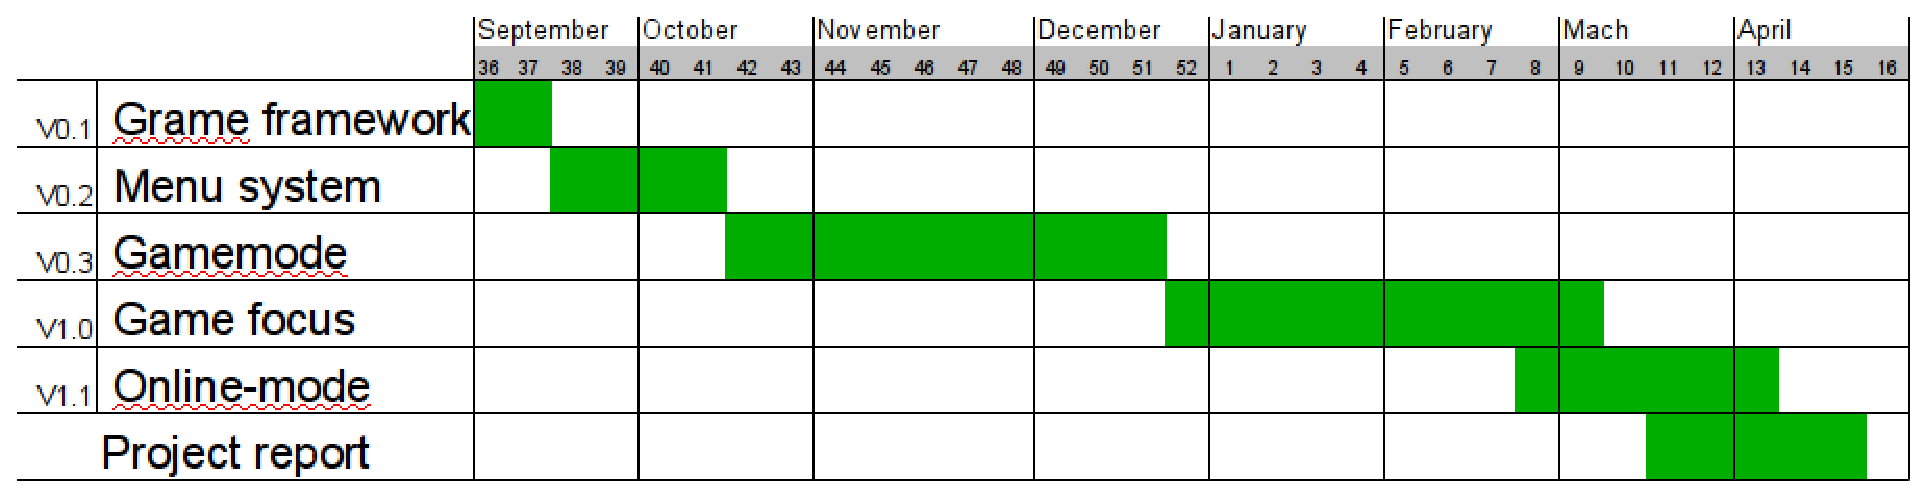
\includegraphics[width=\textwidth]{img/gantt.eps}

\begin{description}
        This was the original time plan, which was followed except for the last three months
\end{description}

\subsection{No hardware acceleration}
% Slow blitting

When i started writing my game i knew that PyGame had support for hardware acceleration. 
Hardware acceleration means that the program can be accelerated by using the computers graphics card instead of solely on the processor.
What i didn't know was that PyGames hardware acceleration is limited to only Windows and even then it is not fully hardware accelerated.

The biggest performance hog in my game is the drawing of every frame to the window.
Since most computers will not support the hardware acceleration though, the game will run easily on almost any computer on lower resolutions, and will run on the monitors native resolution on most desktops.

This is pretty bad performance since the graphics are not advanced at all and not many sprites are in the game.


\subsection{Physics and collision}
% Collision physics troubles

I have previously worked with collision detection and i thought that it was easy to implement.
What i wanted in this game was actual physics, so i simply tried to implement the physics i have learnt in school in programming.
It did seem very easy and implementing the formulas was easy, although there was one thing i was not aware of.
In reality everything moves with a constant speed, but a computer works step by step.
The way to make this as realistic as possible it to have very small iterations of movement on each item, but that would be very resource heavy.

After re-writing my code over 4 times, i finally came up with a acceptable result.
I first moved the object in each direction, and if the speed was faster this frame than it's height or width, it should extra check so it did not jump through an object.
This worked well if one of the objects are static, but if either both objects were moving or if they had a bouncy property it was not as straight forward.

Currently moving objects can easily collide with each other, but i have not been able to make the bounce work as intended.
A object with the bounce property can bounce onto static objects and can be pushed as long as it is not pushed into a wall (If that is the case, the game will crash).



\end{document}
